%%%% Document type  %%%%
\documentclass[preprint,12pt,fleqn]{article}
 \usepackage{ragged2e}
\usepackage{authblk}  % Package for author affiliations
% \usepackage{nopageno} % no page numbers
\usepackage[rightcaption]{sidecap}
\usepackage{placeins} % Floatbarrier

\usepackage[most]{tcolorbox}
\newtcolorbox[auto counter,number within=chapter]{definition}[1][]{
  enhanced,
  breakable,
  fonttitle=\scshape,
  title={Definition \thetcbcounter},
  #1
}

%%%% Document structure %%%%
%\usepackage{geometry}
\usepackage[verbose=true,letterpaper]{geometry}
\geometry{
%    a4paper,
%    left=30mm,
%    right=30mm,
%    top=30mm,
%    bottom=30mm,
    textheight=9in,
    textwidth=6in,
    top=1in,
    headheight=12pt,
    headsep=25pt,
    footskip=30pt,
   % phone  
   %a5paper,
   %width=120mm,
  %height=180mm,
}

\usepackage{lineno} % used along with \linenumbers after begin document. 
\usepackage{setspace} 
\setstretch{1.2}
\makeatletter % The following lines get rid of footer stating pre-preint to elsevier.
\def\ps@pprintTitle{%
\let\@oddhead\@empty
\let\@evenhead\@empty
\def\@oddfoot{}%
\let\@evenfoot\@oddfoot}
\makeatother
\graphicspath{ {../images/} }
\usepackage{pgf} % calculate cohort stats percentage

%%%% Bibliography   %%%%
\usepackage{natbib}
\setcitestyle{numbers,sort&compress}
\setcitestyle{sort&compress}
\usepackage{hypernat} 

%%%% Aesthetics     %%%%
\usepackage{microtype}
% \RequirePackage{times} % Font
\usepackage{ccaption}
\usepackage{siunitx}
\usepackage[T1]{fontenc}
\usepackage[utf8]{inputenc}
\usepackage{nameref}% this allows a reference be named, to print unnumbered references by their section name (used here for linking to Supplemental text in this case).

%%%% Paragraph Formatting %%%
\setlength{\parindent}{2em}
\setlength{\parskip}{6pt plus 2pt minus 1pt}

%%%% Supplemental labels%%%%
%Define command to start a supplemental section
%set the supplemental letter used for figures (e.g. Figure E1)
\newcommand{\beginsupplement}{%
        \setcounter{table}{0}
        \renewcommand{\thetable}{E\arabic{table}}%
        \setcounter{figure}{0}
        \renewcommand{\thefigure}{E\arabic{figure}}%
         }

%%%% Building tables%%%%
\usepackage{booktabs} % required for tables
\usepackage{rotating,tabularx} 
\newcolumntype{Z}{ >{\centering\arraybackslash}X } % defining table content layout per box
\usepackage{ltablex} % allow page break between lines in tabularx
% \usepackage{caption} \captionsetup{font=normalsize} % to set the caption size as normal even when table is tiny.
\usepackage{multirow}
\usepackage{pdflscape}

%%%% Colors %%%%
\usepackage{xcolor} 
\definecolor{natureblue}{RGB}{5,110,210}
    \usepackage[colorlinks]{hyperref} 
\AtBeginDocument{%this allows colours to chage from the defined elsearticle template.
\hypersetup{
    	colorlinks=true,
        linkcolor={natureblue},
    	citecolor={natureblue},
        filecolor=blue!50!black,
        urlcolor=cyan,
    	}}

\definecolor{kispiblack}{HTML}{333333}
\definecolor{kispidarkblue}{HTML}{023047}
\definecolor{kispidarkgreen}{HTML}{006666}
\definecolor{kispired}{HTML}{C70000}
\definecolor{kispilink}{HTML}{007DB8}%219EBC
% \color{kispi_black} %default
\definecolor{kispiblue}{HTML}{701A57}
% City sunset: https://www.color-hex.com/color-palette/40131
\definecolor{colorSUNSET1}{HTML}{eeaf61}
\definecolor{colorSUNSET2}{HTML}{fb9062}
\definecolor{colorSUNSET3}{HTML}{ee5d6c}
\definecolor{colorSUNSET4}{HTML}{ce4993}
\definecolor{colorSUNSET5}{HTML}{6a0d83}
\definecolor{natureblue}{RGB}{5,110,210}    
\usepackage{dirtree}  % Load the dirtree package

% command to use these colors and formatting; xspace for correct spacing including with punctuation marks.
\usepackage{xspace}
\newcommand{\variablesdarkgreen}[1]{\textbf{\textcolor{kispidarkgreen}{#1}}\xspace}
 
\usepackage{tocloft}  % Customizing the Table of Contents
\setcounter{tocdepth}{2}


\usepackage{listings}
\lstset{
    basicstyle=\ttfamily\small,
    breaklines=true,
    postbreak=\mbox{\textcolor{red}{$\hookrightarrow$}\space}, % 
    breakatwhitespace=false,
    % frame=single,
    showstringspaces=TRUE, % Don't show spaces in strings as special characters
    tabsize=2, 
    language=sh 
}

\usepackage{fontspec}
% \setmainfont{IBM Plex Sans}
% \setmonofont{IBM Plex Mono}
% \usepackage{unicode-math}
% \setmathfont{IBM Plex Math}

%\renewcommand{\rmdefault}{ptm}
%\renewcommand{\sfdefault}{phv}


% {{\ttfamily \hyphenchar\the\font=`\-} % set hyphenation for texttt blocks

\usepackage{xpatch}
\xpatchcmd{\AC@deflist}
  {\addtolength{\leftmargin}{\labelsep}}
  {\addtolength{\leftmargin}{\labelsep}\setlength{\itemsep}{0pt}}
  {}{}
\makeatother
\usepackage[printonlyused,withpage,nohyperlinks]{acronym}
%\usepackage{acronym}
% \input{resources/head_phone.tex}
\begin{document}
%\maketitle
% \linenumbers
%\raggedright

\newcounter{myboxcounter}
\newcommand{\boxlabel}[1]{%
  \refstepcounter{myboxcounter}%
  \label{#1}%
}

%\textbf{box~\ref{def:VariantOutcomesDetailed}}.
%\begin{definition}[label=def:VariantOutcomesDetailed]
%\end{definition}\\

\title{Application of qualifying variants for genomic analysis}

% target: Scientific data https://www.nature.com/sdata/author-instructions
% target: Bioinformatics https://academic.oup.com/bioinformatics/

\author[1]{Dylan Lawless\thanks{Addresses for correspondence: \href{mailto:Dylan.Lawless@uzh.ch}{Dylan.Lawless@kispi.uzh.ch}}}
\author[2]{Ali Saadat}
\author[2]{Mariam Ait Oumelloul}
\author[2]{Simon Boutry}
\author[1]{Veronika Stadler}
\author[3]{Sabine Österle}
\author[3]{Jan Armida}
\author[4]{David Haerry}
\author[5]{D. Sean Froese}
\author[1]{Luregn J. Schlapbach}
\author[2]{Jacques Fellay}
%\author[1]{Consortium Members}
\affil[1]{Department of Intensive Care and Neonatology, University Children's Hospital Zürich, University of Zürich, Switzerland.}
\affil[2]{Global Health Institute, School of Life Sciences, École Polytechnique Fédérale de Lausanne, Switzerland.}
\affil[3]{SPHN Data Coordination Center, SIB Swiss Institute of Bioinformatics, Basel, Switzerland.}
\affil[4]{Positive Council, Zürich, Switzerland.}
\affil[5]{Division of Metabolism and Children’s Research Center, University Children’s Hospital Zürich, University of Zurich, Zurich, Switzerland.}


\maketitle
\justify
% \tableofcontents
% \listoffigures
% \listoftables

\clearpage

\begin{abstract}
\noindent
\textbf{Motivation:} \\[1ex]
Qualifying variants (QVs) are genomic alterations selected by defined criteria within analysis pipelines. Although crucial for both research and clinical diagnostics, QVs are often seen as simple filters rather than dynamic elements that influence the entire workflow. While best practices follow variant classification standards and standardised workflows, a unified framework to integrate and optimise QVs for advanced applications is missing.
\\[1ex]
\noindent
\textbf{Results:} \\[1ex]
Our aim is to embed the concept of a ``QV'' into the genomic analysis vernacular, moving beyond a single filtering step. By decoupling QV criteria from other pipeline variables and code, our approach facilitates easier discussion and application.
Our framework, with its new terminology and reference model, offers a flexible approach for integrating QVs into analysis pipelines, thereby enhancing reproducibility, interpretability, and interdisciplinary communication.
A validation case study implementing ACMG criteria in a disease cohort shows that our approach matches conventional methods while offering improved clarity and scalability.
\\[1ex]
\noindent
\textbf{Availability:} \\[1ex]
The source code and data are accessible at \url{https://github.com/DylanLawless/qv2025lawless}. The QV file used in this work is available from
\url{https://doi.org/10.5281/zenodo.15105594} (\texttt{qv\_acmg\_svnindel\_criteria\_20250225.yaml}). The QV framework is available under the MIT licence, and the dataset will be maintained for at least two years following publication.

\end{abstract}

\clearpage

\section*{Acronyms}
\renewenvironment{description}
{\list{}{\labelwidth0pt\itemindent-\leftmargin
    \parsep-1em\itemsep0pt\let\makelabel\descriptionlabel}}
               {\endlist}
\begin{acronym} 
 \acro{acat}[ACAT]{Aggregated Cauchy Association Test }
 \acro{acmg}[ACMG]{American College of Medical Genetics and Genomics}
 \acro{af}[AF]{Allele Frequency}
 \acro{ad}[AD]{Autosomal Dominant}
 \acro{ar}[AR]{Autosomal Recessive}
  \acro{cnv}[CNV]{Copy Number Variant}
 \acro{fair}[FAIR]{Findable, Accessible, Interoperable, and Reusable}
 \acro{gatk}[GATK]{Genome Analysis Tool Kit}
 \acro{gwas}[GWAS]{Genome Wide Association Study}
 \acro{indel}[INDEL]{Insertion / Deletion}
 \acro{iri}[IRI]{Internationalised Resource Identifier}
 \acro{maf}[MAF]{Minor Allele Frequency}
 \acro{ppi}[PPIE]{Public and Patient Involvement and Engagement}
 \acro{prs}[PRS]{Polygenic Risk Score} 
 \acro{qc}[QC]{Quality Control}
 \acro{qv}[QV]{Qualifying variant}
 \acro{rdf}[RDF]{Resource Description Framework}
 \acro{ax}[QV\textsubscript{ax}]{Axiomatic Variants}
 \acro{sf}[SF]{Secondary Findings}
 \acro{sha256}[SHA-256]{Secure Hash Algorithm 256}
 \acro{skat}[SKAT]{sequence kernel association test} 
 \acro{snv}[SNV]{Single nucleotide Variant}
  \acro{snvindel}[SNV/INDEL]{Single Nucleotide Variant / Insertion Deletion}
  \acro{snomedct}[SNOMED CT]{Systematized Nomenclature of Medicine-Clinical Terms}
 \acro{snp}[SNP]{Single Nucleotide Polymorphism}
 \acro{sphn}[SPHN]{Swiss Personalized Health Network}
 \acro{uuid}[UUID]{Universally Unique Identifier}
  \acro{vep}[VEP]{Variant Effect Predictor}
 \acro{vqsr}[VQSR]{Variant Quality Score Recalibration}
 \acro{vsat}[VSAT]{Variant Set Association Test}
 \acro{vus}[VUS]{Variants of Unknown Significance}
 \acro{wgs}[WGS]{Whole Genome Sequencing}
\end{acronym}

\clearpage

\section{Introduction}
\label{sec:intro}

% Background: Define QVs and their role in genomic analysis.
\ac{qv}s are genomic alterations selected by specific criteria within genome processing pipelines, serving as dynamic elements essential for both research and clinical diagnostics. 
\ac{qv}s are not merely static filters applied at a single step in an analysis pipeline; rather, they are dynamic, multifaceted elements that permeate the entire workflow, from initial data quality control to final result interpretation. This nuanced perspective underscores that \ac{qv}s play an integral role in shaping the fidelity and reproducibility of genomic analyses, enabling the iterative refinement of data and facilitating the integration of diverse analytical strategies throughout the pipeline.

% Background/Rationale: Discuss existing practices and identify the gap.
Often, \ac{qv} selection adheres to established variant classification and reporting standards \cite{richards2015standards, li2017standards, li2017intervar, riggs2020technical, tavtigian2020fitting} and standardised workflows \cite{pedersen2021effective, anderson2010data, uffelmann2021genome}. 
However a unified framework for \ac{qv}s is lacking, despite the recognised benefits of similar initiatives, such as \ac{prs} reporting standards \cite{wand2021improving, lambert2021polygenic}.
For instance, tools like vcfexpress \cite{pedersen_vcfexpress_2025} enable flexible, rapid filtering and formatting of VCF files using user-defined expressions. The application of independently defined \ac{qv} criteria would complement such tools.
This role is particularly important for reproducibility across distributed computing environments \cite{bal_programming_1989} and would also integrate with workflow managers such as Snakemake \cite{molder_sustainable_2021} or Nextflow \cite{di_tommaso_nextflow_2017}, streamlining genomic processing tasks.

% Background: Outline the variability in QV selection and provide examples.
The criteria for \ac{qv} selection vary by application. 
For example, \ac{gwas} may focus on common variants, while clinical analyses usually target rare or known pathogenic variants. 
Previous studies have demonstrated the utility of \ac{qv}s \cite{povysil2019rare, cirulli2015exome}, yet no common approach exists. 
Here, we detail four typical applications of \ac{qv} sets:
\begin{enumerate}
    \item \textbf{\ac{qv} passing \ac{qc} only}: Generates large datasets (e.g. > 500,000 variants per subject) for \ac{gwas} or initial \ac{wgs} pre-processing.
    \item \textbf{Flexible \ac{qv}}: Balances between \ac{qc} and false positives, yielding intermediate datasets (e.g. fewer than 100,000 variants per subject) for uses such as rare variant association testing.
    \item \textbf{\ac{qv} for rare disease}: Applies stringent filtering to produce smaller datasets (e.g. < 1,000 variants per subject), targeting known genes or single causal variants.
    \item \textbf{Known disease panel \ac{qv} set}: Focuses on well-established gene panels with pathogenic variants (e.g. the \ac{acmg} \ac{sf} set) for clinical reporting \cite{miller2023acmg}.
\end{enumerate}

% Background/Rationale: Emphasise the importance of careful QV selection.
 These examples illustrate a few common applications without providing an exhaustive classification of all possible \ac{qv} uses.
The careful selection and categorisation of \ac{qv}s are thus critical for accurate reporting and reproducibility, sometimes even more so than the choice of the analysis pipeline itself \cite{olson2023variant}.

% Background: Address the increasing need for diverse QV protocols in large-scale sequencing.
As \ac{wgs} becomes standard for large cohorts \cite{lee2018gene, jansen2019genome}, the integration of diverse \ac{qv} protocols is critical for data cleaning and analysis. 
During sequencing analysis several layers can be responsible for triggering \ac{qv} protocols, including
pre-existing metadata, technical \ac{qc} results, and post-calling annotations,
highlighting the need for a clear, unified approach. 

% Framework: Present the proposed solution.
We propose treating the \ac{qv} as a standalone entity, independent from other pipeline variables. We suggest structured human- and machine-readable criteria, aligned with FAIR principles \cite{wilkinson2016fair} to facilitate integration across databases \cite{van2023bridging, toure2023fairification}. We advocate for the use of standard vocabularies, unique identifiers, and flexible file formats to support this integration.

\section{Methods}
\subsection{Implementation} \label{sec:framework}

%By introducing a new vocabulary and a standard reference model for \ac{qv}s, we aim to clarify the concept and improve communication and methodological discussion across disciplines for more advanced tasks.
Implementation configurations and roles within analysis pipelines include, for example:
theoretical pipelining of \ac{qv} sets,
establishing public or standardised \ac{qv} sets for specific analytical scenarios, and 
recognition that \ac{qv}s are integral throughout the analysis pipeline rather than confined to a single end-stage.
We introduce a simple framework for the effective use of \ac{qv} protocols, comprising four components as illustrated in \textbf{Figure \ref{fig:qv_pipeline_with_file_vcurrent_guru_case_study_result} (A)}:

\begin{itemize}
    \item \textbf{1. Variables}: The criteria variables sourced as part of the pipeline (see \textbf{Box \ref{box:acmg_criteria_yaml}}).
    \item \textbf{2a. Technical description}: An optional narrative detailing each step within the overall \ac{qv} set (see \textbf{Box \ref{box:acmg_criteria_yaml}}).
    \item \textbf{2b. \ac{ppi} description}: An optional narrative providing a patient-focused interpretation of the protocol, incorporating preferences and priorities.
    \item \textbf{3. \ac{qv} set ID}: A unique identifier that links analysis records.
    \item \textbf{4. Source code}: The implementation of the variables file within the pipeline code, for example through custom scripts or workflow managers.
\end{itemize}

We propose the \ac{qv} set ID as a unique identifier linking variant sets used in analyses. This facilitates integration into databases,
by representing data in formats such as \ac{rdf} schemas \cite{toure2023fairification}, and allows for features including \ac{sha256} hash functions, \ac{uuid}s, semantic combinations, \ac{iri} incorporation, registry-based allocation, and standard mapping such as \ac{snomedct}. The results can be used alongside other genomic-specific concepts spanning from sample processing to the sequencing run \cite{van2023bridging}.

This framework efficiently manages \ac{qv}-specific variables (e.g. allele frequency thresholds) separately from general pipeline settings, ensuring clarity and specificity. Its versatile format supports applications across genomic analyses and by linking the \ac{qv} set ID to both results and raw data sources in a database for downstream interpretation and reporting.

\subsection{Example application of qualifying variants in WGS analysis}

Multiple \ac{qv} protocols can be combined to generate progressively filtered datasets tailored to specific analytical needs. Often, different \ac{qv} sets are applied sequentially, with the final outcomes merged to address distinct objectives. For instance, a comprehensive analysis pipeline might integrate:
\begin{itemize}
  \item \colorbox{kispiblue!05}{\texttt{QV SNV/INDEL}}  \ac{snvindel},
  \item \colorbox{kispiblue!05}{\texttt{QV CNV}} \ac{cnv},
  \item \colorbox{kispiblue!05}{\texttt{QV structural variation}},
  \item \colorbox{kispiblue!05}{\texttt{QV rare disease known}}, and 
  \item \colorbox{kispiblue!05}{\texttt{QV statistical association \ac{qc}}}.
\end{itemize}
The final analysis yields (1) a joint cohort disease association (e.g. variant P-values) and (2) individual single-case results (e.g. clinical genetics diagnosis for a patient)
\cite{auwera_genomics_2020, li2025statistical}.
As an example, in 
\textbf{Figure \ref{fig:qv_pipeline_with_file_vcurrent_guru_case_study_result} (A)}
we focus on a SNV/INDEL pipeline employing two \ac{qv} sets:
\colorbox{colorSUNSET2!20}{\texttt{QV SNV INDEL 1}} for flexible cohort-level filtering, and 
\colorbox{colorSUNSET2!20}{\texttt{QV SNV INDEL 2}} for stricter filtering in subsequent single-case analysis. The pipeline is illustrated in \textbf{Box \ref{box:pipe}}, and can be summarised as follows:

``A cohort of patient WGS data was analysed to identify genetic determinants for phenotype X. Initially, a flexible \ac{qv} set was applied using the 
\colorbox{colorSUNSET1!10}{\texttt{pipeline DNA SNV INDEL v1}}, which implements the \colorbox{colorSUNSET2!20}{\texttt{QV SNV INDEL 1}} criteria to produce the prepared dataset (\colorbox{colorSUNSET3!10}{\texttt{dataset DNA SNV INDEL v1}}). This dataset was then analysed alongside other modules (e.g. \colorbox{colorSUNSET4!10}{\texttt{PCA SNV INDEL v1}} and \colorbox{colorSUNSET5!10}{\texttt{statistical genomics v1}}) to derive a cohort-level association signal (Result 1). Next, the same prepared dataset was re-filtered with the stricter \colorbox{colorSUNSET2!20}{\texttt{QV SNV INDEL 2}} criteria to identify known causal variants for each patient, yielding the final dataset (\colorbox{colorSUNSET3!10}{\texttt{dataset DNA SNV INDEL v2}}) and resulting in individual case reports (Result 2).''

\begin{tcolorbox}[
    colback=white!0,
    colframe=black,
    boxrule=1pt,
    arc=1mm,
    outer arc=1mm,
    title=\textbf{\refstepcounter{myboxcounter}\label{box:pipe}Box \themyboxcounter: Example diagrammatic representation}
]
\dirtree{%
.1 \colorbox{colorSUNSET1!10}{\texttt{pipeline DNA SNV INDEL v1}}.
.2 Flexible \ac{qv} criteria.
.3 \colorbox{colorSUNSET2!20}{\texttt{QV SNV INDEL 1}} $\rightarrow$ \colorbox{colorSUNSET3!10}{\texttt{dataset DNA SNV INDEL v1}}.
.4 \colorbox{colorSUNSET4!10}{\texttt{PCA SNV INDEL v1}}.
.4 \colorbox{colorSUNSET5!10}{\texttt{statistical genomics v1}} $\rightarrow$ Result 1.
.3 \colorbox{colorSUNSET3!10}{\texttt{dataset DNA SNV INDEL v1}}.
.4 Rare disease \ac{qv} criteria.
.5 \colorbox{colorSUNSET2!20}{\texttt{QV SNV INDEL 2}} $\rightarrow$ \colorbox{colorSUNSET3!10}{\texttt{dataset DNA SNV INDEL v2}}.
.6 \colorbox{colorSUNSET5!10}{\texttt{single case report SNV INDEL v1}} $\rightarrow$ Result 2.
.3 Joint analysis output.
}
\medskip

Joint analysis output from:\\
Result 1 = Cohort-level association signal (e.g. variant P-value).\\
Result 2 = Single variant report per patient.
\end{tcolorbox}

\subsection{Usage in a Validation Study}

In a validation study, we demonstrate the use of our \ac{qv} criteria framework 
% achieve a 100\% match in criterion application when 
compared to the conventional manual approach. 
This analysis was performed on an in-house rare disease cohort of 940 individuals, which had been pre-processed for \ac{qc}. % and filtered using a minimal \ac{qv} test set.
We used genome-wide set of variants which was filtering to target rare varaints (\ac{maf} $< 0.01$) restricted to known disease genes based on the Genomics England panel ``Primary immunodeficiency or monogenic inflammatory bowel disease,'' retrieved using our PanelAppRex R repository (\url{https://github.com/DylanLawless/PanelAppRex}) 
\cite{lawless_panelapprex_2025}. 
This provided us with a prepared dataset of 6026 candidate variants annotated with 376 information sources.
The dataset was prepared in R using GuRu, our variant interpretation tool that consolidates all annotation sources and scores variants as candidate causal, and was imported from gVCF format as output by \ac{vep}.

%Initially, we implemented an \ac{acmg} variant classification protocol \cite{richards2015standards} manually. 
%We then re-implemented the same protocol using the new framework for \ac{qv} criteria in YAML format. 
We selected the first eight \ac{acmg} criteria for assigning pathogenicity scores to variants \cite{richards2015standards}; six of these were relevant for this cohort. First, the analysis was performed manually by hard-coding each criterion in the pipeline script, reflecting a typical workflow. Second, the same criteria were imported from the \ac{qv} YAML file for the new framework approach, using the file ``qv acmg svnindel criteria 20250225.yaml'' (see \textbf{Box \ref{box:acmg_criteria_yaml}} or \url{https://doi.org/10.5281/zenodo.15105594}).
The outputs from both methods were captured and compared.

Additional details of the YAML criteria in this \ac{qv} set included definitions for \texttt{ACMG\_PS1} (identifying previously established pathogenic amino acid changes), \texttt{ACMG\_PS3} (supporting functional studies with matching inheritance patterns), and \texttt{ACMG\_PS5} (covering compound heterozygosity with high-impact variants). The criteria for \texttt{ACMG\_PM2} and \texttt{ACMG\_PM3} assess variant frequency and in trans occurrences, respectively, while \texttt{PS2} and \texttt{PS4} were not applicable to this cohort.

% Individual steps within the \ac{qv} criteria can be further classified for organisational purposes using simple labels such as ``QC'' and ``filter''. For example, filtering thresholds (e.g. allele frequency > 0.1 in a cohort, < 0.1 in gnomAD) may be applied directly to exclude variants, while annotation-based criteria (e.g. QC flags) might not remove variants outright but instead inform downstream analyses that integrate multiple \ac{qv} filters.

\begin{tcolorbox}[
    colback=white!0,
    colframe=black,
    boxrule=1pt,
    arc=1mm,
    outer arc=1mm,
    title=\textbf{\refstepcounter{myboxcounter}\label{box:acmg_criteria_yaml}Box \themyboxcounter: qv\_files/acmg\_criteria.yaml}
]
\begin{verbatim}
qv_set_id: acmg_sf_v3.2

acmg_pvs1:
  description_technical: >
    Null variants (IMPACT = HIGH) in genes where 
    loss-of-function causes disease.
    Includes homozygous variants, dominant inheritance, 
    and compound heterozygous cases.
    Compound heterozygosity is considered when both 
    variants are HIGH impact. WARNING: Not phase checked.
  logic: "or"
  conditions:
    - condition:
        field: IMPACT
        value: "HIGH"
        operator: "=="
...
shasum -a 256 acmg_criteria.yaml | fold -w 32
d91fde41a5fff48631adecba38773d61
9ae8cd5cff9b9b42ef7f5efbd6bbfcdf
acmg_criteria.yaml
\end{verbatim}
\end{tcolorbox}


\section{Results}
\subsection{Validation Case Study}

We validated our \ac{qv} protocol using \ac{acmg}-based criteria for a rare disease cohort of 940 individuals. 
We then conducted the variant classification using two approaches: a conventional manual method with hard-coded criteria, and our new YAML-based implementation
As shown in \textbf{Figure \ref{fig:qv_pipeline_with_file_vcurrent_guru_case_study_result} (B)}, 
the outputs from both methods were identical, demonstrating a 100\% match. This confirmed that our framework of a standalone, shareable, \ac{qv} criteria file can be imported and applied programmatically with equivalent accuracy, providing a reproducible resource that is adaptable across different pipelines and programming environments.

% Results/Methods: Figure showing pipeline and validation case study.
\begin{figure}[!h]
\centering
\begin{minipage}{0.85\textwidth}
\raggedright A\\[0.5ex]
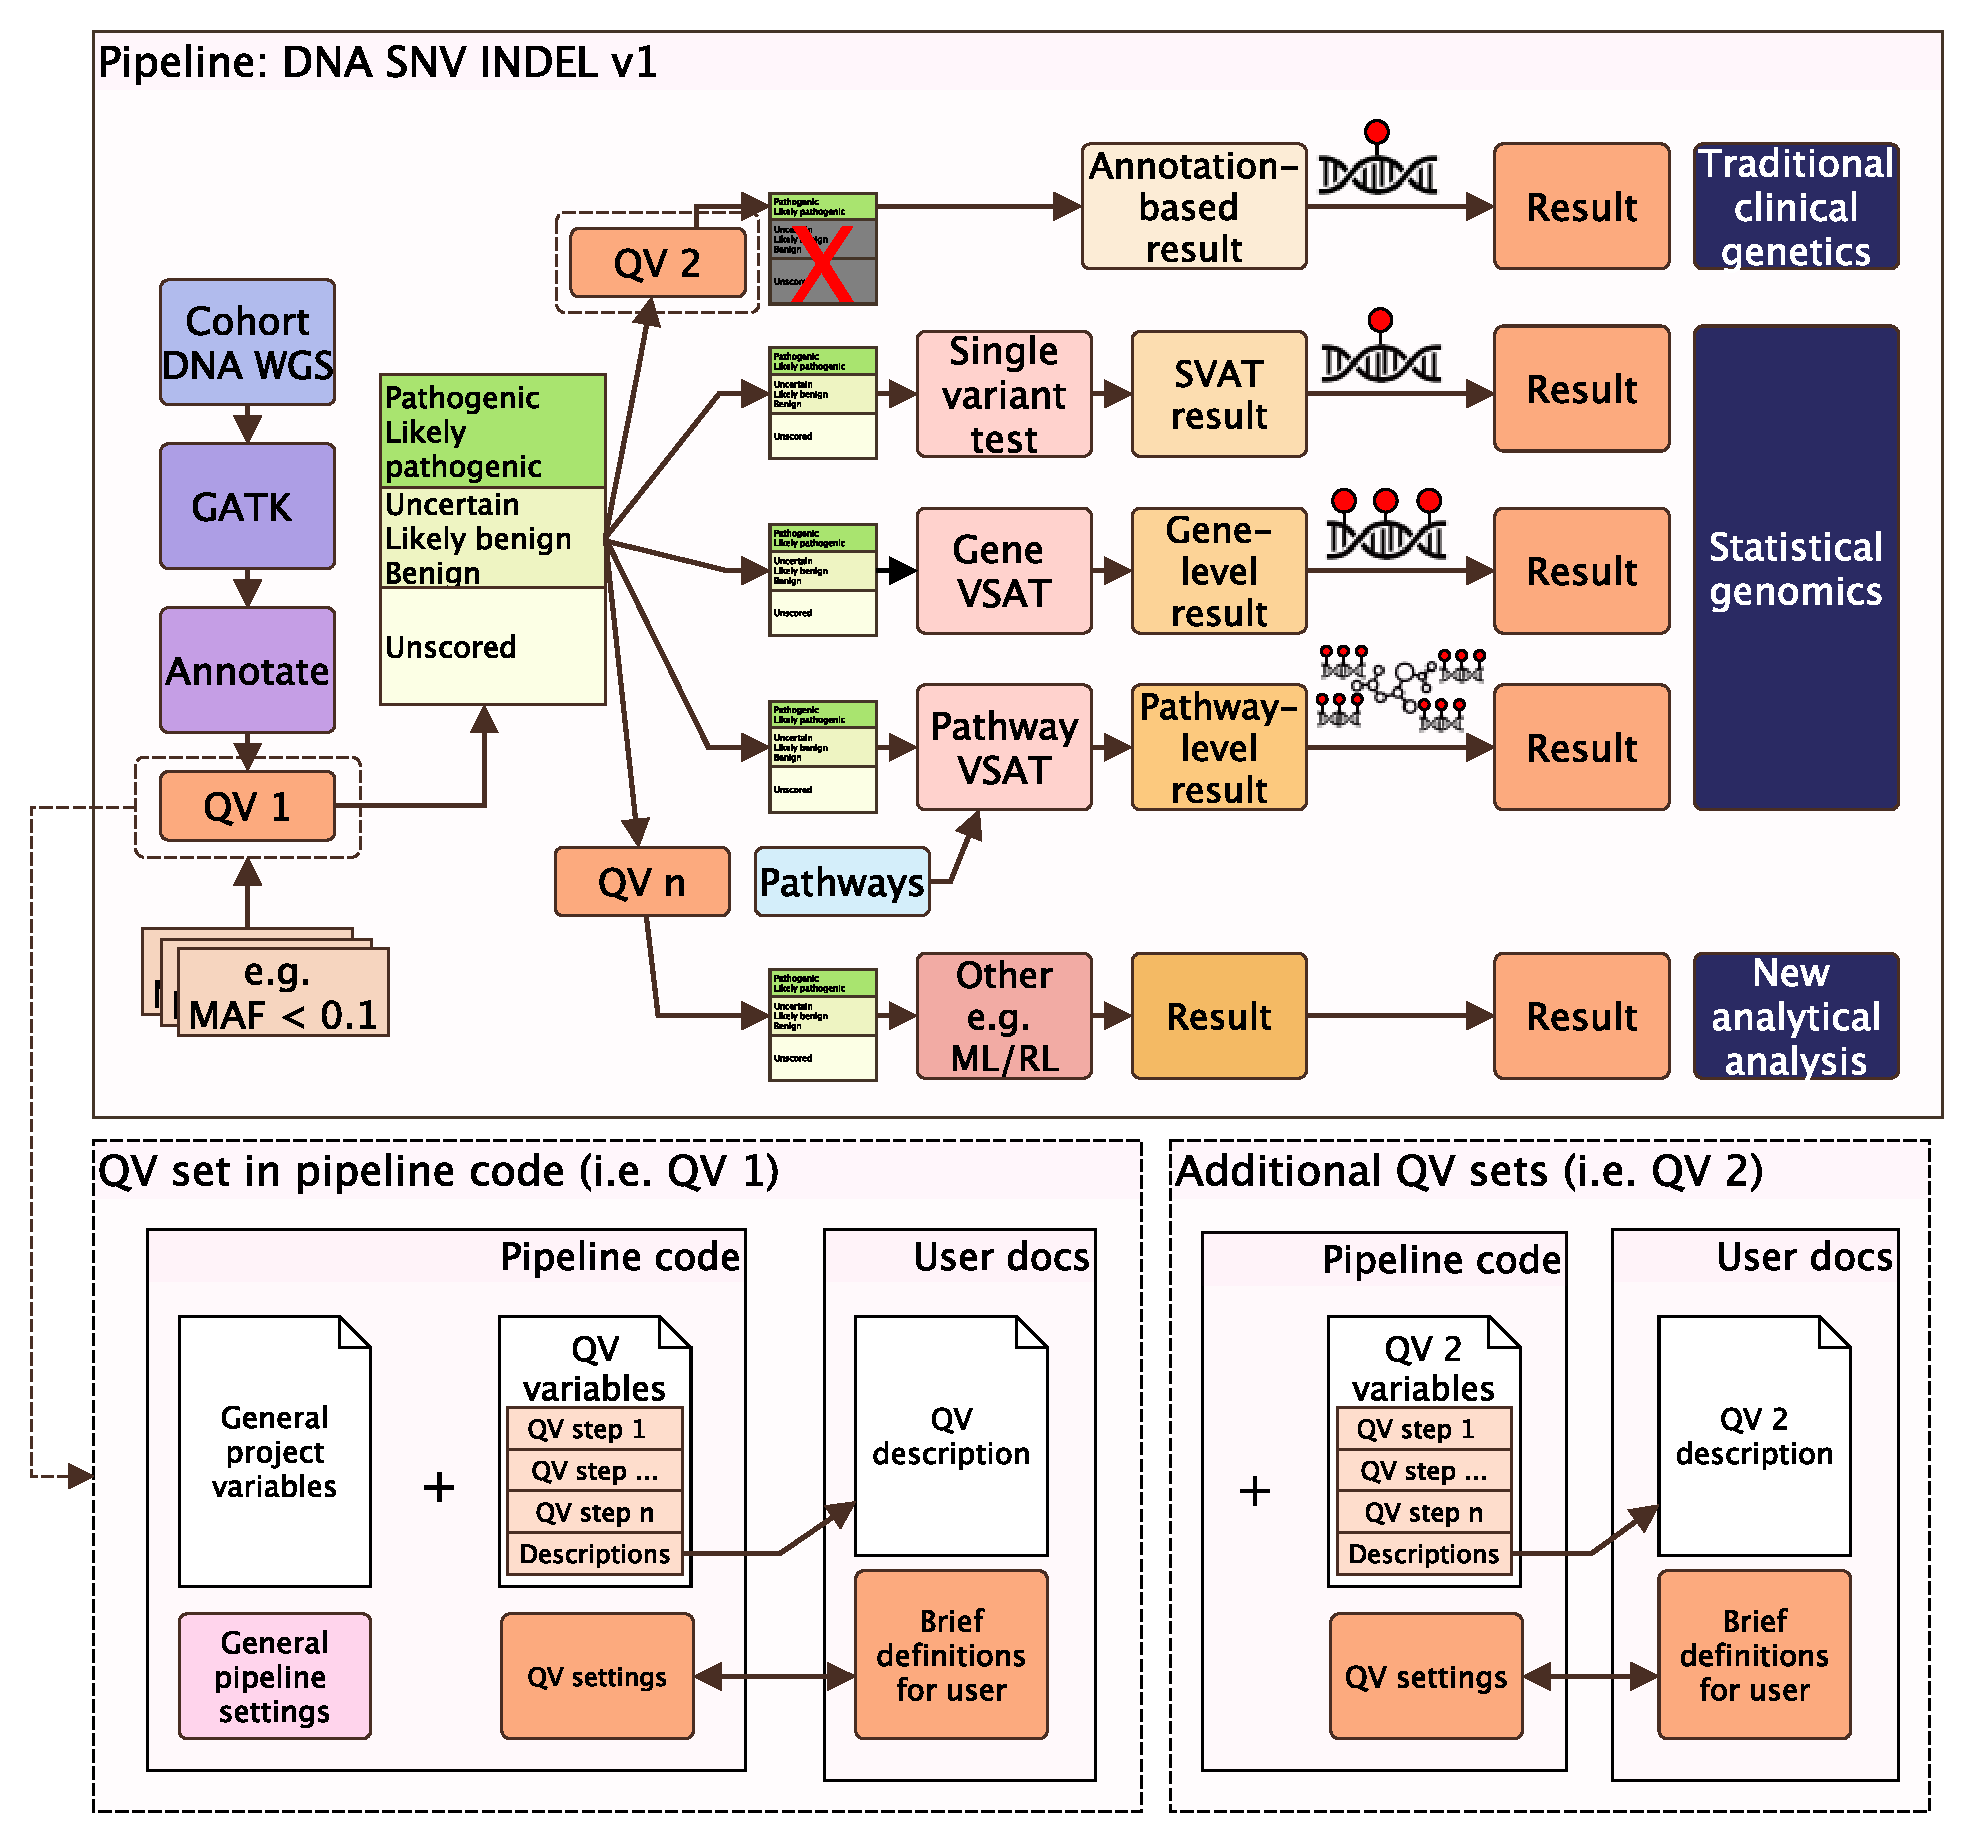
\includegraphics[width=\textwidth]{./images/qv_pipeline_with_file_vcurrent.pdf}
\end{minipage}\\[-2ex]
\begin{minipage}{0.9\textwidth}
\raggedright B\\[0.5ex]
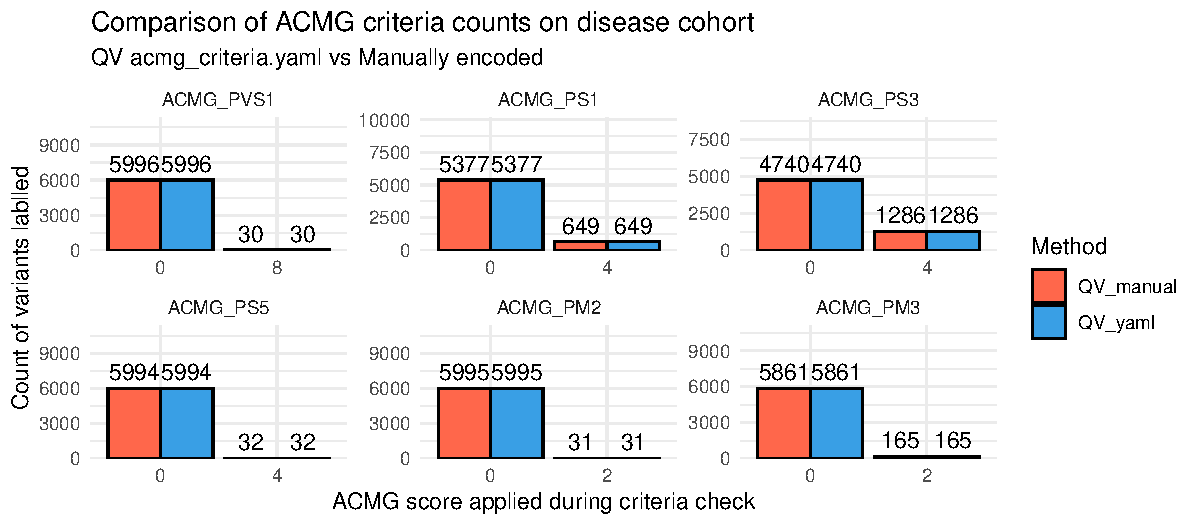
\includegraphics[width=\textwidth]{./images/Guru_singlecase_validation_of_yaml_vs_manual.pdf}
\end{minipage}
    \caption{Summary of the QV application for a WGS pipeline. In panel (A), \ac{qv}1 and \ac{qv}2 are presented as sequentially piped protocol steps. In this example, \ac{qv}2 differs from \ac{qv}1 by retaining only likely/pathogenic variants (indicated by a red X). The QV file loaded by the analysis pipeline comprise a description field (optional) and a variables field (mandatory). The \ac{qv} criteria may be spread throughout the pipeline.
    (B) Validation case study using an \ac{acmg} criteria subset, demonstrating a 100\% match between manually encoded and standalone YAML-based \ac{qv} (\texttt{qv\_files/acmg\_criteria.yaml}) for assigning pathogenicity scores.}
    \label{fig:qv_pipeline_with_file_vcurrent_guru_case_study_result}
\end{figure}

\subsection{Implications}
% Framework: Highlight the clinical relevance and benefits.
In the validation study, we applied \ac{acmg} criteria for variant interpretation. In clinical genetics, for instance, the resulting output can be used to retrieve candidate pathogenic variants using \ac{acmg} scoring methods \cite{richards2015standards, tavtigian2020fitting}.
Application of additional \ac{qv} sets, such as the widely used \ac{acmg} \ac{sf} set for clinical reporting \cite{miller2023acmg}, can be used to confirm any secondary findings.

In a clinical setting it is necessary to bridge the gap between technical detail and lay understanding. By explicitly documenting variant qualifying criteria and making \ac{qv} data accessible, our framework builds trust and supports meaningful \ac{ppi} \cite{morris_answer_2011}. The \ac{qv} file adapts by integrating the main criteria variables with optionally dedicated fields for both technical description and \ac{ppi} description. This approach captures the analysis intent defined by the \ac{qv} set creator and embeds patient preferences from the start. 

For example, patient preferences recorded in the \ac{ppi} description can be automatically incorporated into a genetic report without additional interpretation, ensuring clarity and consistency throughout the analysis. This transparency guarantees that both experts and laypersons receive information in a format suited to their needs, thereby improving diagnostic traceability and accelerating the translation of genetic research into clinical practice.

\FloatBarrier

\section{Summary}
This paper introduces a framework for integrating qualifying variants into genomic analysis pipelines, enhancing reproducibility, interpretability and the seamless translation of research findings into clinical practice.

\section{Funding}
This project was supported through the grant Swiss National Science Foundation  320030\_201060, and NDS-2021-911 (SwissPedHealth) from the Swiss Personalized Health Network and the Strategic Focal Area `Personalized Health and Related Technologies' of the ETH Domain (Swiss Federal Institutes of Technology).

\section{Acknowledgements}
Acknowledgements We would like to thank all the patients and families who have been providing advice on SwissPedHealth and its projects, as well as the clinical and research teams at the participating institutions.

\section{Contributions}
DL designed the work and contributed to the manuscript.
AS, SB, VS, DH, SÖ, JA contributed to the manuscript.
JF, SF, LJS supervised the work, manuscript, and applied for funding.

\section{Competing interests}
The authors declare no competing interests.

\section{Ethics statement}
Summary statistics were used from studies which have been previously reported and approved by the respective ethics committees of all participating centers (Cantonal Ethics Committee Bern, approval number KEK-029/11) and the study was conducted in accordance with the Declaration of Helsinki.

\bibliographystyle{unsrtnat}
\bibliography{references} 

\end{document}
